% geni_3.tex - GENI Lab 2 for Cloud Computing class (Spring 2015)
% Chanmann Lim - April 2015

\documentclass[a4paper]{article}

\usepackage[margin=1 in]{geometry}
\usepackage{listings}
\usepackage{graphicx}
\usepackage{float}

\begin{document}
\title{CS 7001-03: Report for GENI Lab 3 - QoS Configuration and Load Balancing using Software-Defined Networking}
\author{Chanmann Lim\\ 
	\texttt{cl9p8@mail.mail.missouri.edu}}
\date{April 14, 2015}
\maketitle

% ---------------------------------------- 1 ----------------------------------------
\paragraph{1. } Screenshots taken in Step 3.4:
\begin{figure}[H]
  \centering
    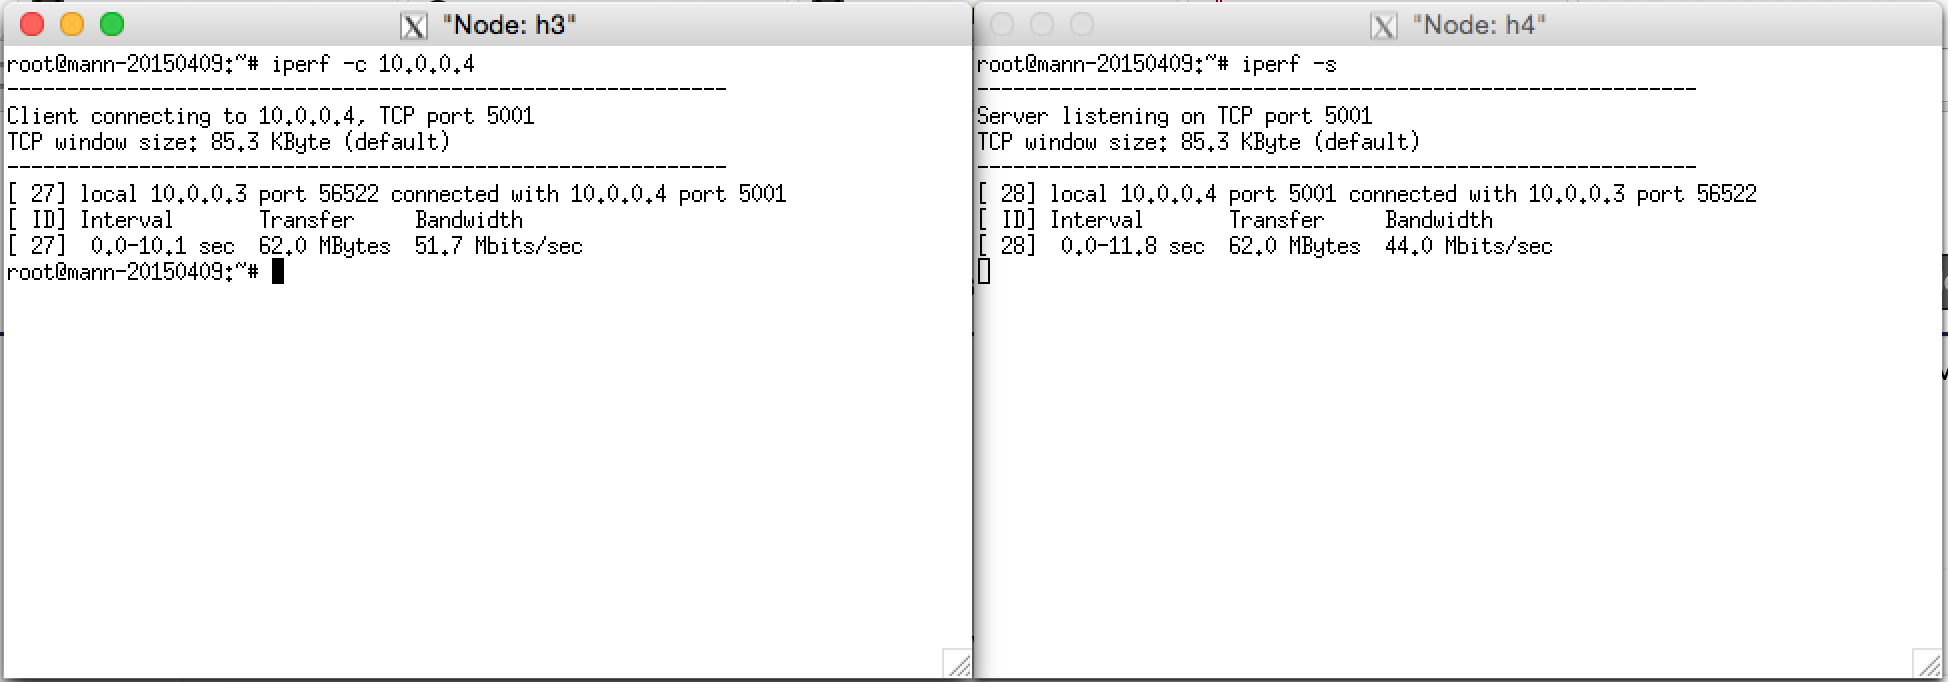
\includegraphics[scale=.47]{iperf_h3_h4.png}
  \caption{Iperf test from h3 to h4}
\end{figure}
\begin{figure}[H]
  \centering
    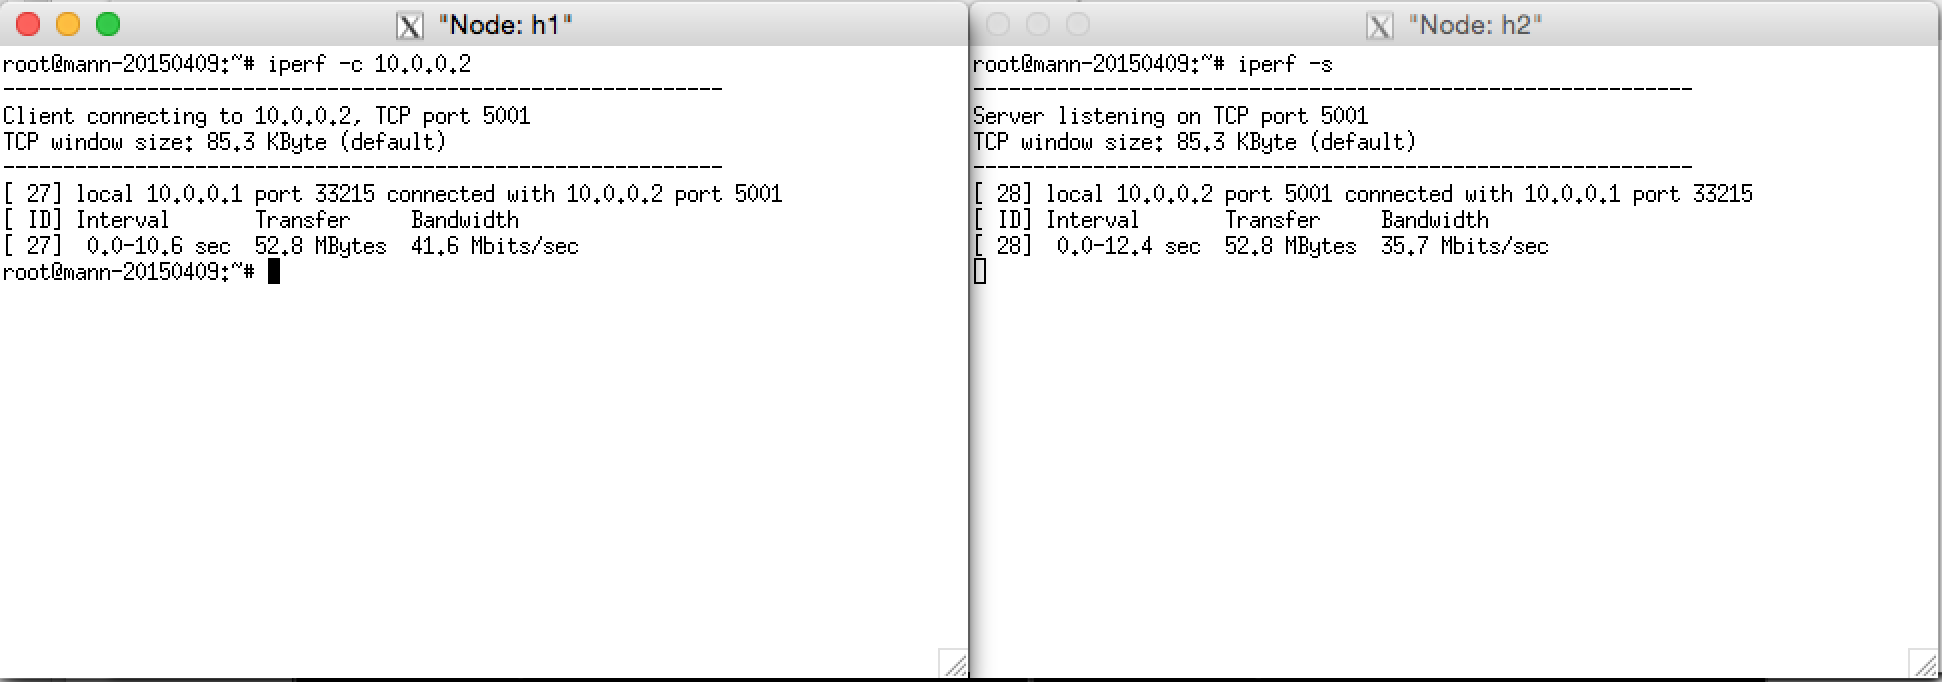
\includegraphics[scale=.47]{iperf_h1_h2.png}
  \caption{Iperf test from h1 to h2}
\end{figure}

The packets captured by Wireshark with "lo" interface and "of" filter in \textbf{step. 3.4} list only the OpenFlow control packet of the loopback interface, and when clicking on an "of\_aggregate\_stats\_request" packet, we obtain the detail OpenFlow headers in the packet such as \emph{version}, \emph{type}, \emph{length}, \emph{xid}, \emph{stats\_type}, \emph{flags}, \emph{of\_match}, \emph{table\_id}, and \emph{out\_port}.

And the \emph{of\_match} header contains \emph{wildcards}: Wildcards fields, \emph{in\_port}: Input switch port, \emph{eth\_src}: Ethernet source address, \emph{eth\_dst}: Ethernet destination address, \emph{vlan\_vid}: Input VLAN id, \emph{vlan\_pcp}: Input VLAN priority, \emph{eth\_type}: Ethernet frame type, \emph{id\_dscp}: IP ToS (actually DSCP field, 6 bits), \emph{ip\_proto}: IP protocol or lower 8 bits of ARP opcode, \emph{ipv4\_src}: IP source address, \emph{ipv4\_dst}: IP destination address, \emph{tcp\_src}: TCP source port, \emph{tcp\_dst}: TCP destination port.


% ---------------------------------------- 2 ----------------------------------------
\paragraph{2. } Screenshot of Iperf test from host4 to host1:
\begin{figure}[H]
  \centering
    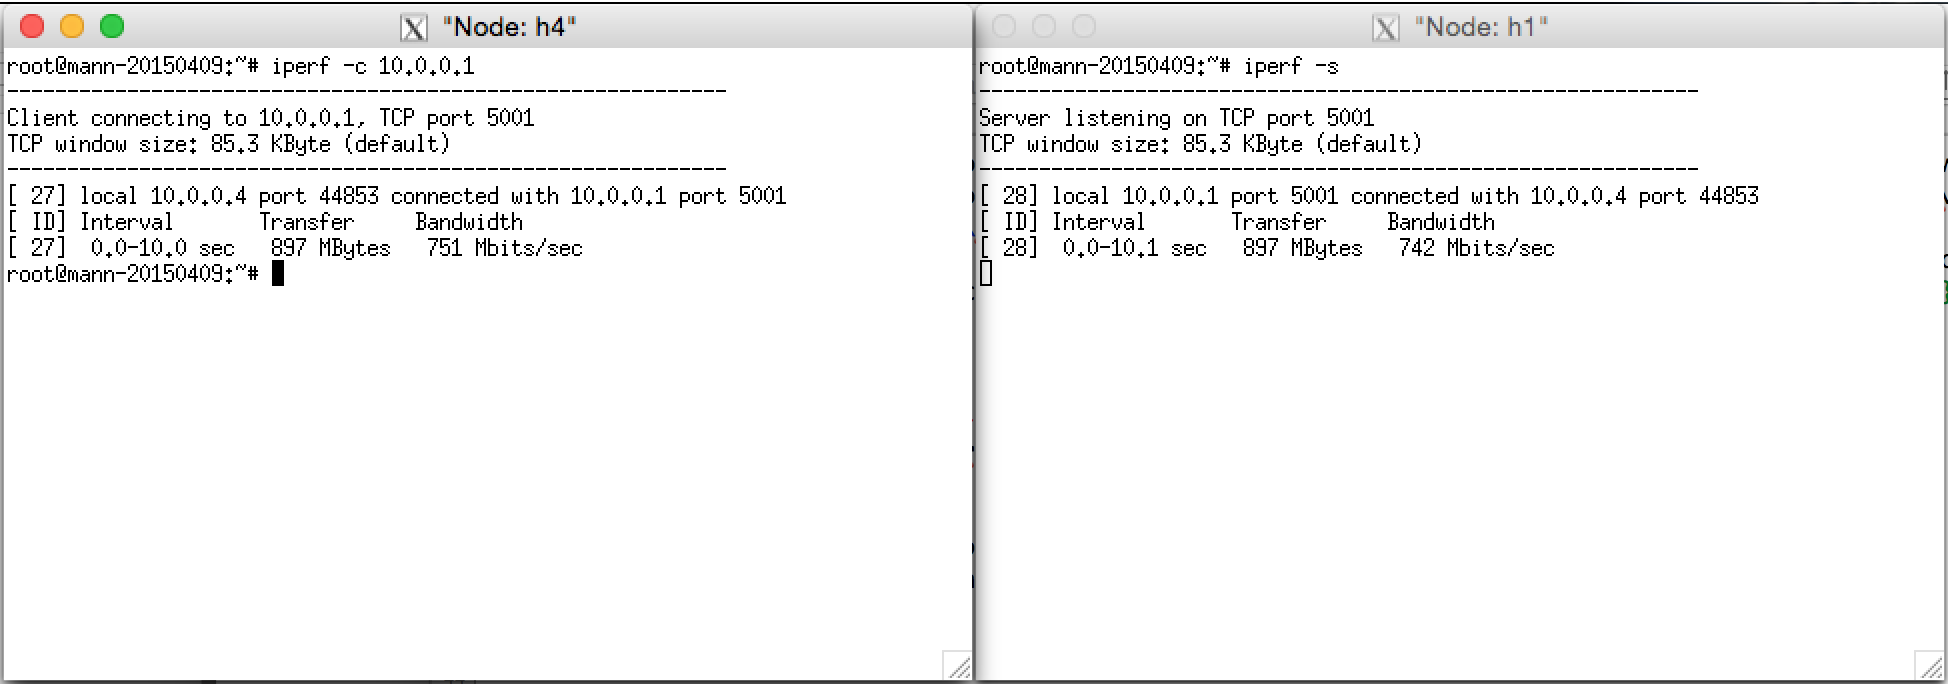
\includegraphics[scale=.47]{iperf_h4_h1.png}
  \caption{Iperf test from h4 to h1}
\end{figure}

By using the topology created in \textbf{step 3.3.1} and the QOS configuration in \textbf{step 3.3.2}, the traffic flow between host4 and host1 is conducted through queue "0" which had configured with the maximum bandwidth up to 1 Gbps, similarly since the traffic flow from host2 to host1 doesn't match with both queue "1" and queue "2"'s rules "50Mbps-h3-h4" and "40Mbps-h1-h2" respectively it will fallback to use queue "0" in the switches.


% ---------------------------------------- 3 ----------------------------------------
\paragraph{3. } Assuming that we have the topology with 6 hosts, 7 switches and 1 controller as shown in the Figure 14 of the GENI Lab 3 instruction. To establish a new queue 'q3' of 80 Mbps between host 'h5' as source and host 'h6' as destination, first we need to configure the queue by editing the \texttt{mininet-add-queues.py}

\begin{verbatim}
# vim /home/floodlight-qos-beta/apps/qos/mininet-add-queues.py
\end{verbatim}
then change the \texttt{queuecmd} variable at line 67 to \\

\small{\sf{queuecmd = "sudo ovs-vsctl \%s \--\-- \--\--id=@defaultqos create qos type=linux-htb other-config:max-rate=1000000000 queues=0=@q0,1=@q1,2=@q2,3=@q3 \--\-- \--\--id=@q0 create queue other-config:min-rate=1000000000 other-config:max-rate=1000000000 \--\-- \--\--id=@q1 create queue other-config:max-rate=50000000 \--\-- \--\--id=@q2 create queue other-config:max-rate=40000000 \--\-- \--\--id=@q3 create queue other-config:max-rate=80000000 other-config:min-rate=2000000" \% config\_strings[sw]}} \\

\noindent then run:
\begin{verbatim}
# ./floodlight-qos-beta/apps/qos/mininet-add-queues.py
\end{verbatim}

It will configure queue "1", queue "2", and queue "3" with 50 Mbps, 40 Mbps and 80 Mbps respectively for all ports of all switches. Next change directory to \texttt{floodlight-qos-beta/apps/qos/} and execute \texttt{qospath2.py} command to establish flow between 'h5' and 'h6' using queue "3"
\begin{verbatim}
# ./qospath2.py -p 8080 -a -N 80Mbps-h5-h6 -J '{"eth-type":"0x0800","queue":"3"}' \
   -S 10.0.0.5 -D 10.0.0.6
\end{verbatim}

% ---------------------------------------- 4 ----------------------------------------
\paragraph{4. } Two screenshots taken in Step 3.5:
\begin{figure}[H]
  \centering
    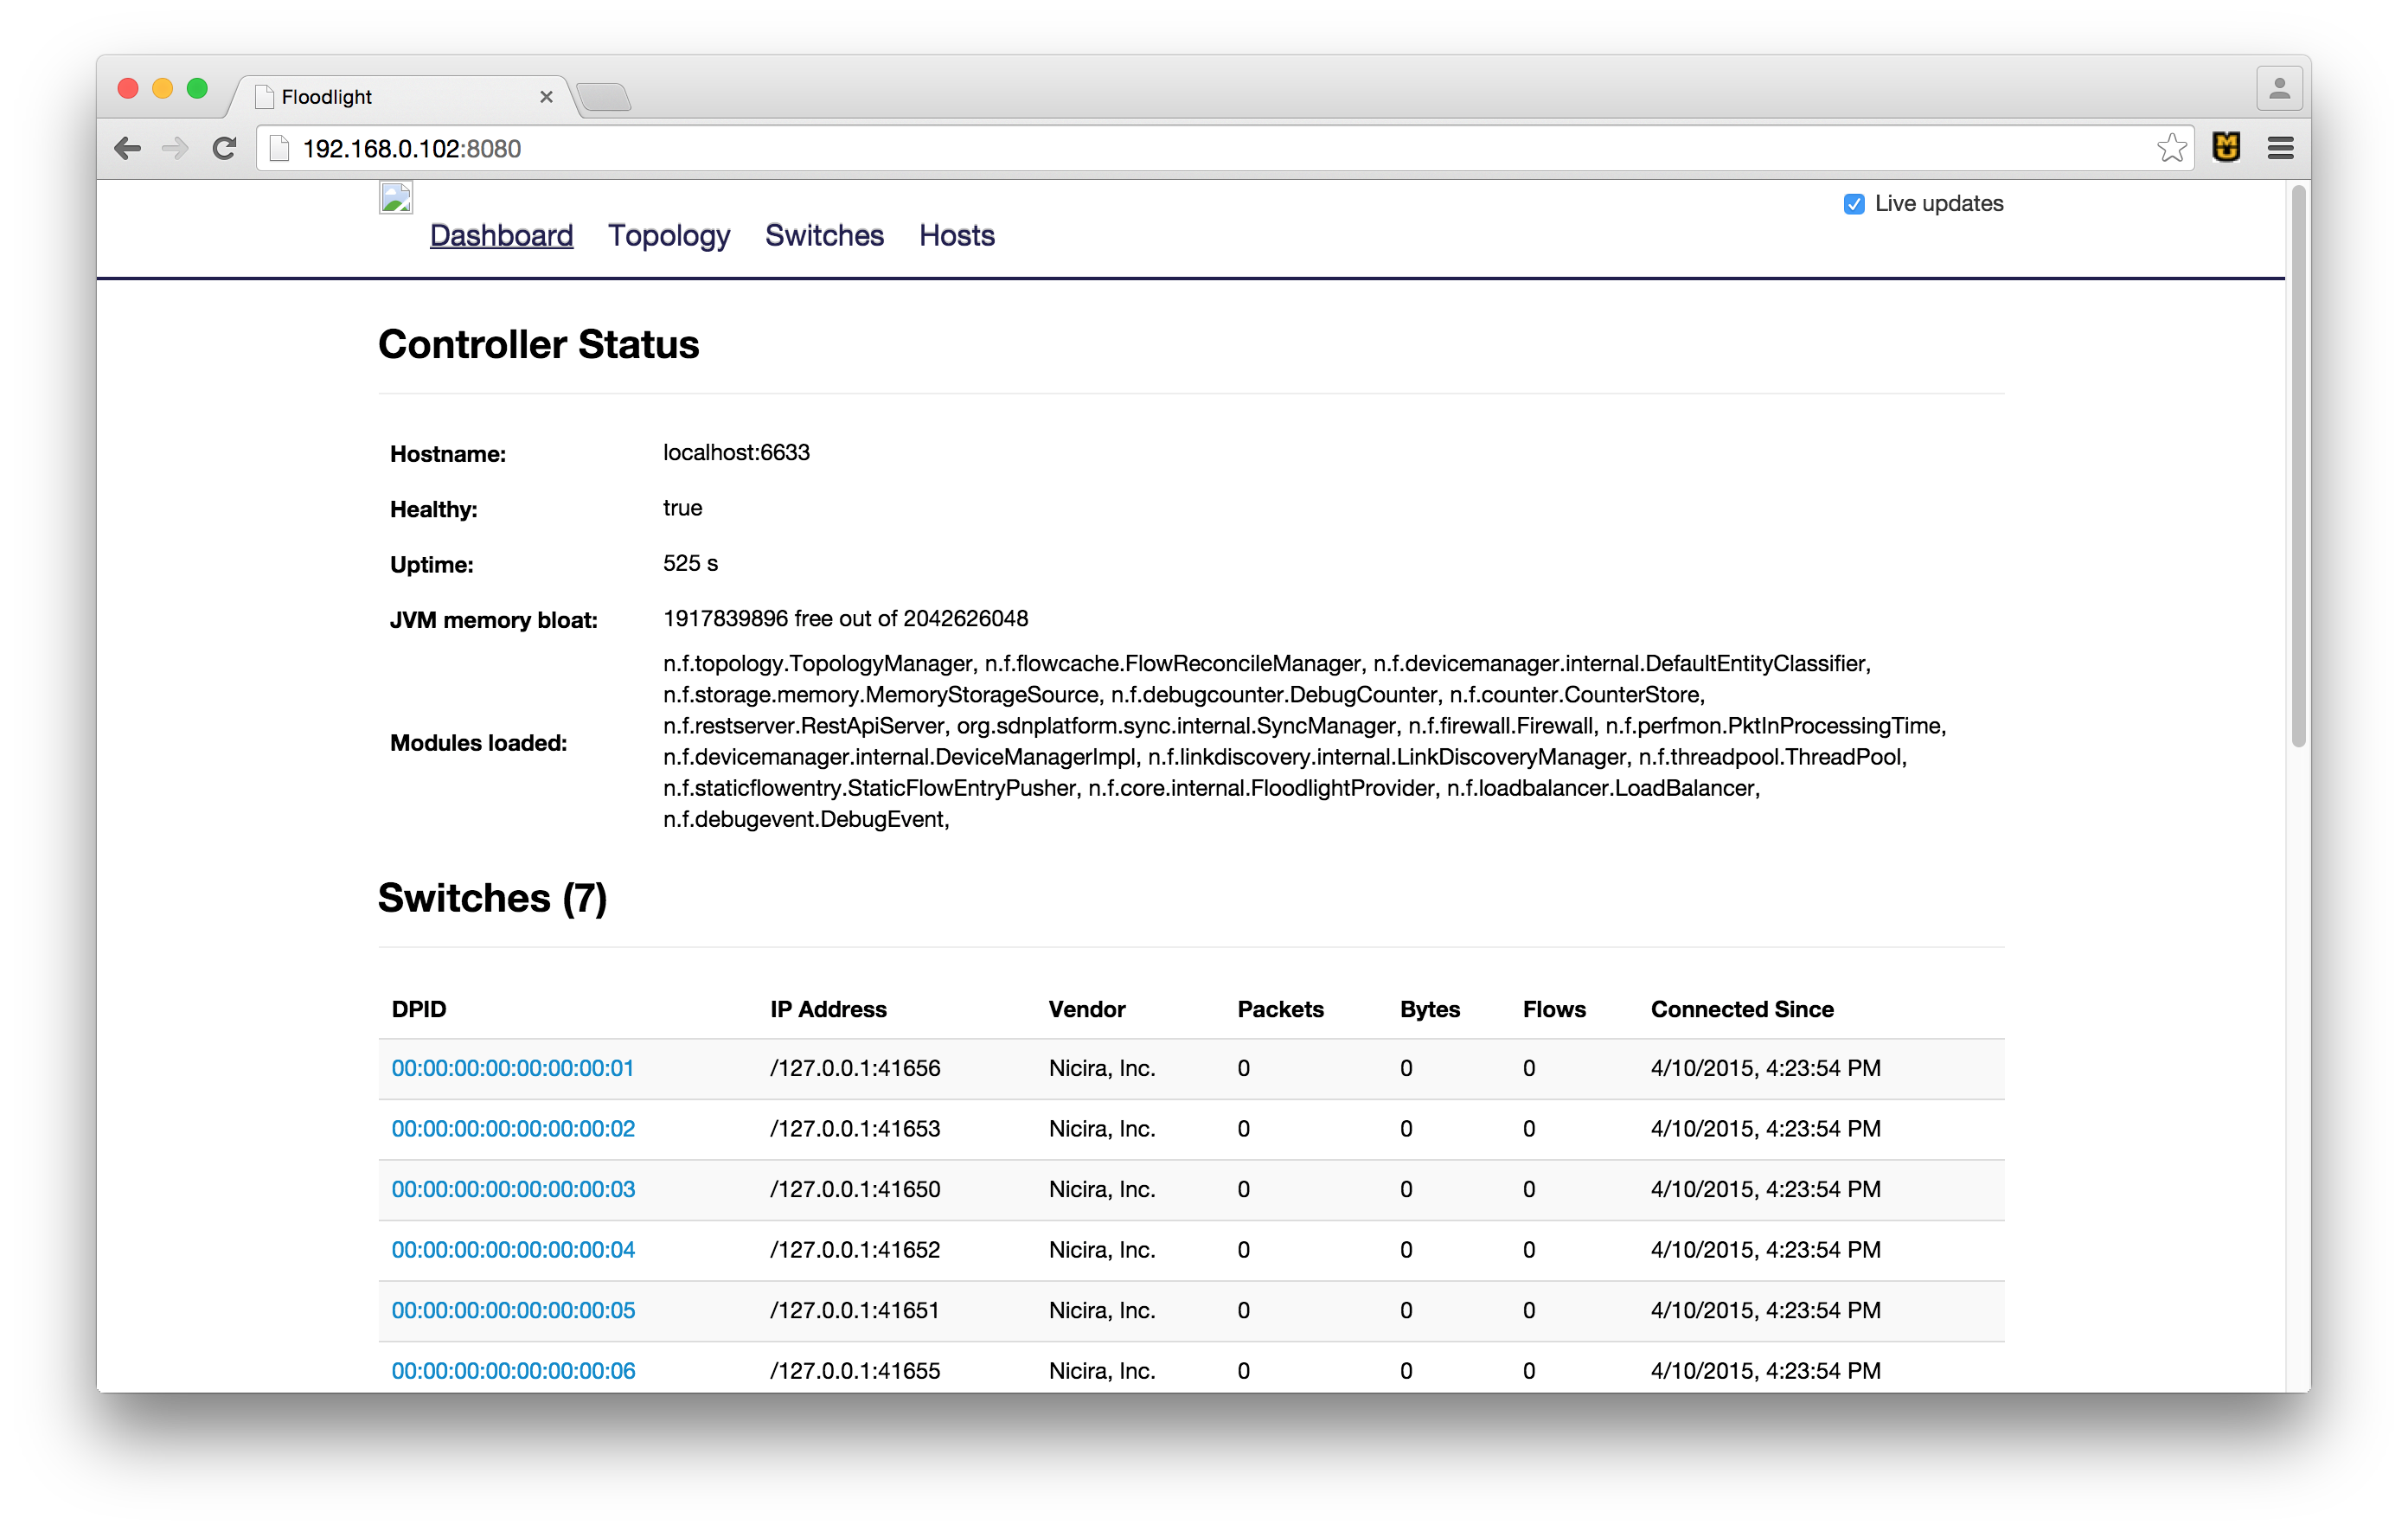
\includegraphics[scale=.34]{floodlight_ui.png}
  \caption{Floodlight with LoadBalancer module loaded}
\end{figure}
\begin{figure}[H]
  \centering
    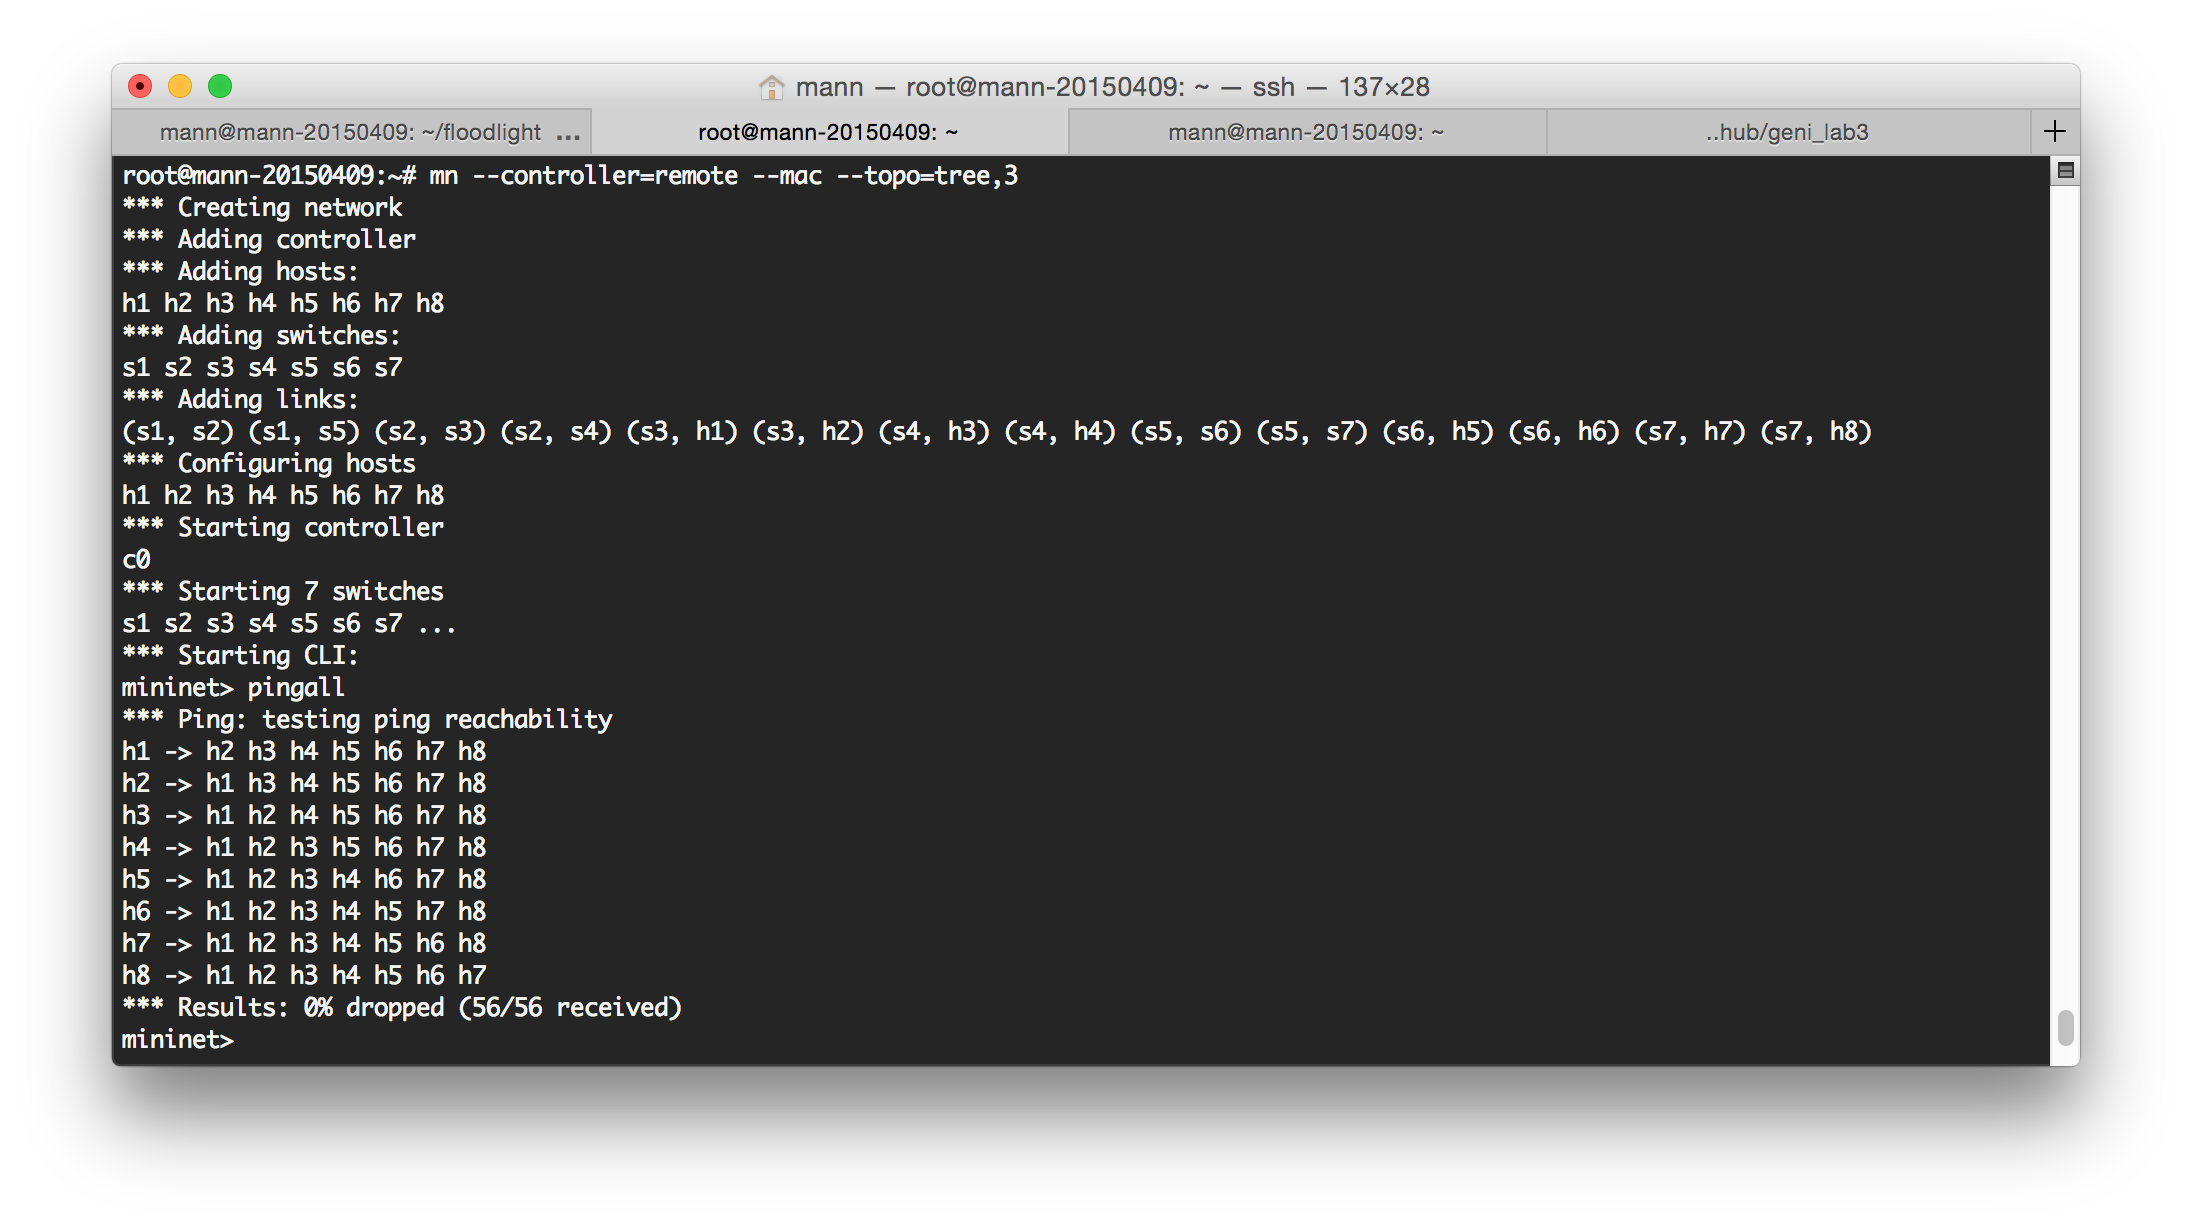
\includegraphics[scale=.44]{pingall.png}
  \caption{minute pinball in 'tree,3' topology}
\end{figure}

% ---------------------------------------- 5 ----------------------------------------
\paragraph{5. } This question requires that you extend the load\_balancer.sh script and run new Load Balancer Experimentation using the following steps: \\

i) Scale the load balancer to handle more requests by adding two new hosts h5 (10.0.0.5) and h6 (10.0.0.6) to the load balancer pool and adding the appropriate entries in the load\_balancer.sh script. Run the load\_balancer.sh script again to update the new flow rules. \\

ii) On the mininet CLI, start the xterm terminals for the new end-hosts h7 and h8 by giving the below command: \$mininet: xterm h7 h8 \\

iii) Start the ping command from hosts h1 and h2 terminals to load balancer 10.0.0.100 and allow the ping to run continuously. Simultaneously, start the ping command from hosts h7 and h8 terminals to the load balancer 10.0.0.100. \\

What happens when you ping from new end-hosts h7 and h8 to the load balancer 10.0.0.100? Which hosts are responding to the new requests and what does this result suggest? Attach a single screenshot with all the four ping windows running simultaneously.
\end{document}